\documentclass[12pt,a4paper]{report}
\usepackage[utf8]{vietnam}\usepackage{amsmath, amsthm, amssymb,latexsym,amscd,amsfonts,enumerate}
\usepackage[top=3.5cm, bottom=3.0cm, left=3cm, right=3.0cm]{geometry} 
\usepackage{color, fancyhdr, graphicx, wrapfig}
\usepackage[unicode]{hyperref}
\usepackage[vietnamese]{babel}
\usepackage{amsthm}
\usepackage{amsmath}
\usepackage{amsfonts}
\usepackage{amssymb}
\usepackage{graphicx} 
\usepackage{titling}
\usepackage{secdot}
\usepackage{enumitem}
\usepackage{tikz}
\usepackage{array}
\usetikzlibrary{calc}
\usepackage{longtable}
\usepackage{indentfirst}
\usepackage{fancyhdr}
\usepackage{exscale,relsize,makeidx}
%\usepackage{refcheck}

\setcounter{tocdepth}{4}
\setcounter{secnumdepth}{4}
\newtheorem{dn}{Định nghĩa}[chapter]
\newtheorem{tc}{Tính chất}[chapter]
\newtheorem{dl}{Định lý}[chapter]
\newtheorem{md}{Mệnh đề}[chapter]
\newtheorem{bd}{Bổ đề}[chapter]
\newtheorem{hq}{Hệ quả}[chapter]
\newtheorem{nx}{Nhận xét}[chapter]
\newtheorem{vd}{Ví dụ}[chapter]
\newtheorem{cy}{Chú ý}[chapter]
\pagenumbering{roman}\pagestyle{plain}
%\pagestyle{fancy}
%\lhead{\it \changefontsizes{11pt}Luận văn thạc sĩ:}
%\rhead{\it Một số phương pháp vô hướng hóa cơ bản trong tối ưu đa mục tiêu}
%\lfoot{\it Nguyễn Văn Vân } 			         
%\rfoot{\it K19.2 trường ĐHSG}
\renewcommand{\headrulewidth}{1,2pt} 			
\renewcommand{\footrulewidth}{1,2pt}

\newcommand{\dstc}[2]
{
	\newdimen\stringwidth\setbox0=\hbox{#1}
	\stringwidth=\wd0
	\hspace*{-\parindent}\hspace*{.5\textwidth}\hspace*{-.5\wd0}#1\hfill #2\bigskip
	
}  
\usepackage{scrextend}
\fancyhf{}
\lhead{}
\chead{\thepage}
\rhead{}
\cfoot{}
\rfoot{}
\lfoot{}
\pagestyle{fancy}
\renewcommand{\headrulewidth}{1pt}

%\changefontsizes{13pt}

\begin{document} 
	\begin{titlepage}
		\begin{tikzpicture}[remember picture, overlay]
			\draw[line width = 1.5pt] ($(current page.north west) + (1in,-1in)$) rectangle ($(current page.south east) + (-0.6in,1in)$);
			
		\end{tikzpicture}
		\centering
		\textbf{ỦY BAN NHÂN DÂN THÀNH PHỐ HỒ CHÍ MINH\smallskip\\
			TRƯỜNG ĐẠI HỌC SÀI GÒN}\par
		\rule{5cm}{0.5pt}\par
		\vspace{2cm}
		{\Large\textbf{NGUYỄN VĂN XXX}\par}
		\vspace{4cm}
		{\Large\textbf{MỘT SỐ XXX \\ VÔ HƯỚNG HÓAXXX\\ 
				TRONG TỐI ƯU XXX }\par}
		\vspace{4cm}
		\large\textbf{ ĐỀ TÀI NGHIÊN CỨU KHOA HỌC SINH VIÊN }\par		
		
		\large{CHUYÊN NGÀNH: TOÁN ỨNG DỤNG}
		\vspace{1.5cm}
		
		\vfill
		\textbf{Thành phố Hồ Chí Minh, năm 2021}
	\end{titlepage}
	\begin{titlingpage}
		\begin{tikzpicture}[remember picture, overlay]
			\draw[line width = 1.5pt] ($(current page.north west) + (1in,-1in)$) rectangle ($(current page.south east) + (-1in,1in)$);
			
		\end{tikzpicture}
		\centering
		\textbf{ỦY BAN NHÂN DÂN THÀNH PHỐ HỒ CHÍ MINH\smallskip\\
			TRƯỜNG ĐẠI HỌC SÀI GÒN}\par
		\rule{5cm}{0.5pt}\par
		\vspace{2cm}
		{\Large\textbf{NGUYỄN VĂN XXX}\par}
		\vspace{4cm}
		{\Large\textbf{MỘT SỐ XXX \\ VÔ HƯỚNG HÓAXXX\\ 
				TRONG TỐI ƯU XXX }\par}
		\vspace{4cm}
		\large\textbf{ ĐỀ TÀI NGHIÊN CỨU KHOA HỌC SINH VIÊN }\par		
		
		\large{CHUYÊN NGÀNH: TOÁN ỨNG DỤNG}
		\vspace{1.5cm}
		
		\large\textbf{Người hướng dẫn} \par
		\vspace{2cm}
		
		\large\textbf{XXXX}\par
		
		%	\includegraphics[height=2cm]{chukynew}
		\vfill
		\textbf{Thành phố Hồ Chí Minh, năm 2021}
	\end{titlingpage}
	
	%\large
	\renewcommand{\baselinestretch}{1.2}
	\fontsize{13pt}{20pt}\selectfont
	
	\chapter*{Lời cam đoan}
	\thispagestyle{fancy}
	\addcontentsline{toc}{chapter}{Lời cam đoan}
	\vspace{1cm}
	\indent
	
	Tôi tên là Nguyễn Văn Vân, Sinh viên lớp...., khoa.... , khóa ....,  thuộc trường Đại học Sài Gòn. Tôi xin cam đoan rằng: Toàn bộ nội dung được trình bày trong bản báo cáo này này đều do chính tôi thực hiện dưới sự hướng dẫn của thầy.... Những kết quả nghiên cứu của tác giả khác được sử dụng trong đề tài  đều có trích dẫn đầy đủ. Tôi xin hoàn toàn chịu trách nhiệm nếu có các nội dung sao chép không hợp lệ hoặc vi phạm quy chế đào tạo. 
	\\
	\\
	\\
	\rightline{{\it {Tp. HCM, tháng 10 năm 20XX}} \hspace*{0cm}}
	\rightline{\textbf{Tác giả} \hspace*{2cm}}
	\\
	\\
	\\
	
	%\vspace*{1cm}
	\rightline{\textbf{Nguyễn Văn XX}\hspace*{1.2cm}}
	
	\chapter*{Lời cảm ơn}
	\thispagestyle{fancy}
	\addcontentsline{toc}{chapter}{Lời cảm ơn}
	\vspace{1cm}
	\indent
	
	Luận văn này được hoàn thành tại trường Đại Học Sài Gòn dưới sự hướng dẫn của XXXXXXX. Nhóm thực hiện đề tài chúng em  xin bày tỏ lòng biết ơn chân thành và sâu sắc về sự tận tâm và nhiệt tình của Thầy trong suốt quá trình tác giả thực hiện đề tài
	
	
	\bigskip
	Xin cám ơn Phòng Đào tạo  và Khoa Toán - Ứng dụng trường Đại học Sài Gòn đã tạo nhiều điều kiện thuận lợi, giúp chúng em hoàn thành nhiệm vụ học tập.
	\\
	\\
	\\
	\rightline{{\it {Tp. HCM, tháng 10 năm 2021}} \hspace*{0cm}}
	\rightline{\textbf{Các tác giả} \hspace*{2cm}}
	\\
	\\
	
	%\vspace*{1cm}
	\rightline{\textbf{Nguyễn Văn XXX} \hspace*{1.2cm}}
	\newpage
	
	\addcontentsline{toc}{chapter}{Mục lục}
	\tableofcontents
	%\thispagestyle{plain}
	\chapter*{Danh mục các kí hiệu}
	\thispagestyle{fancy}
	\addcontentsline{toc}{chapter}{Danh mục các kí hiệu}
	\begin{longtable}{l l}
		
		$\mathbb{R}$ & Tập các số thực\\
		%$\emptyset $ & Tập rỗng\\
		$\mathbb{R}^n$ & Không gian Euclide $n$-chiều\\
		${\rm co}(S)$ & Bao lồi của tập $S$\\
		${\rm cl}(S)$ & Bao đóng của tập $S$\\
		${\rm bd}(S)$ & Biên của tập $S$\\
		$\mathrm{cone}(S)$ & Nón sinh bởi tập $S$\\
		$\mathrm{conv}(S)$ & Nón lồi sinh bởi tập $S$\\
		${\rm int}(S)$ & Phần trong của tập $S$\\
		${\rm epi}(f)$ & Trên đồ thị của $f$\\
		$|| x ||$ & $\sqrt {x_1^2 + x_2^2 + \ldots + x_n^2 }$		\\
		$[x,y]$ & Đoạn thẳng nối 2 điểm $x$ và $y$\\
		$F$ & Tập chấp nhận được của bài toán tối ưu\\
		$\langle u, v \rangle$ & Tích vô hướng của hai véc tơ $u$ và $v$ trong $\mathbb{R}^n$\\
		$\alpha S$ & Tập hợp $	\left\{ {x \in \mathbb{R}^n \mid x = \alpha s,s \in S} \right\}$\\
		dom$f$ & Miền hữu hiệu của $f$\\
		$\nabla f\left( x \right)$ & Véc tơ gradient của hàm $f$\\
		$\partial f(z)$ & Dưới vi phân của hàm lồi $f$\\
		$N(C,z)$ & Nón chuẩn của $C$ tại điểm $z$
		
	\end{longtable}
\newpage
\pagenumbering{arabic} 
\chapter*{Lời nói đầu}
\thispagestyle{fancy}
\addcontentsline{toc}{chapter}{{\bf  Lời nói đầu}\rm}
\renewcommand{\baselinestretch}{1.2}
Khi giải quyết những vấn đề tối ưu trong thực tế, người ta thường phải quan tâm giải quyết đồng thời nhiều mục tiêu khác nhau. Những vấn đề như thế thường gặp trong kinh tế hoặc trong các bài toán khoa học, kỹ thuật.

Đối với bài toán đơn mục tiêu, việc xác định nhiệm vụ tìm cực đại hay cực tiểu của hàm mục tiêu là vấn đề khá rõ ràng. Trong khi đó, với nhiều mục tiêu đang quan tâm trên cùng một tập xác định, rất ít khi xảy ra việc các mục tiêu đạt được đồng thời cực đại hay cực tiểu. Điều này đòi hỏi phải xác định rõ ý nghĩa của việc  tìm cực đại hay cực tiểu trong tối ưu đa mục tiêu.  Hiển nhiên giữa các mục tiêu ấy còn có các mối liên quan hay có các sự thỏa hiệp nào đó.

Một phương pháp đơn giản nhất được áp dụng khi cần tối ưu  nhiều mục tiêu đang quan tâm là xác định cho mỗi mục tiêu một trọng số thích hợp, rồi từ đó chuyển bài toán nhiều mục tiêu bằng bởi mục tiêu trung bình cọng của  các mục tiêu thành phần đã xác định trọng số. Phương pháp như thế gọi là phương pháp tối ưu hóa đa mục tiêu bằng tổng các mục tiêu theo trọng số, hay nói gọn là phương pháp tổng có trọng số.

Xét bài toán tối ưu đa mục tiêu có dạng:
$$
\begin{array}{lll}
	{\rm (MP)}& {\rm Min}& (f_1(x),\ldots,f_m(x))\\
	&&x \in A.
\end{array}
$$
với  $ f_{1}(x),...,f_{m}(x)$  là các hàm mục tiêu thành phần xác định trên $\mathbb{R}^n$ và $A \subset \mathbb{R}^n$ là miền ràng buộc. Giả sử  ứng với mục tiêu thứ $j, j = 1,...,m,$ có  trọng số $\theta _j$, với $\theta _j \in \left[0,1 \right]$ và $\sum\limits_{j = 1}^m \theta _j  = 1$. Khi đó, thay vì bài toán (MP), người ta quan tâm bài toán đơn mục tiêu có hàm mục tiêu là trung bình cộng các mục tiêu theo trọng số, đó là,
$$
\begin{array}{lll}
	{\rm (SMP)}& {\rm Min}& \theta_1f_1(x)  + ... + \theta _m f_m(x)\\
	&&x \in A.
\end{array}
$$


Việc chuyển một bài toán đa mục tiêu về bài toán đơn mục tiêu gọi chung là phương pháp vô hướng hóa tối ưu đa mục tiêu.


Câu hỏi được đặt ra là:  Giữa bài toán $\mathrm{(MP)}$  và ${\rm (SMP)}$  có mối liên hệ nghiệm như thế nào? Ngoài phương pháp tổng trọng số như trên còn có phương pháp nào khác.

Đề tài này hướng đến việc tìm hiểu và hệ thống lại một số phương pháp đã biết trong tối ưu hóa đa mục tiêu ngoài phương pháp tổng trọng số. Cụ thể,  ngoài việc tìm hiểu về phương pháp tổng trọng số, luận văn còn tìm hiểu thêm các phương pháp khác như  Phương pháp Chankong-Haimes, Phương pháp Hybrid. Ngoài ra, luận văn cũng quan tâm thêm một số phương pháp vô hướng hóa mở rộng trong  tối ưu đa mục tiêu.


Luận văn được tìm hiểu dưới tên gọi

{\it ``Một số phương pháp vô hướng hóa cơ bản trong tối ưu đa mục tiêu''.}


Dựa trên cơ sở lý thuyết về Tối ưu hóa và Tối ưu đa mục tiêu, các phương pháp trên được tìm hiểu thông qua các  mô hình hóa  cụ thể. Từ đó,  mối quan hệ nghiệm giữa bài toán đa mục tiêu và bài toán vô hướng  hóa được khảo sát. Luận văn cũng giới thiệu các ví dụ để minh họa các mối quan hệ nghiệm giữa hai bài toán đó. Ngoài ra, xem như là phần mở rộng của các phương pháp vô hướng hóa tối ưu đa mục tiêu, luận văn này cũng nghiên cứu thêm 2 phương pháp khác dùng trong tối ưu hóa đa mục tiêu đó là: Phương pháp tối ưu theo thứ tự từ điển và Phương pháp tối ưu theo thứ tự Max.





 Ngoài phần mở đầu, kết luận và danh mục các tài liệu tham khảo, luận văn được tổ chức thành 3 chương. Trong đó: 

$\bullet$ Chương 1: Bao gồm các kiến thức chuẩn bị, nội dung có liên quan đến một số kiến thức cơ bản về Lý thuyết tối ưu đơn mục tiêu và  đa mục tiêu. Phần này được tham khảo từ các tài liệu  \cite{Son1} và \cite{Son2}.

$\bullet$ Chương 2: Tìm hiểu các phương pháp vô hướng hóa đã được đề cập trong phần giới thiệu. Các kiến thức của chương này chủ yếu được khảo cứu từ các tài liệu \cite{Mat}, \cite{Joel}. Các định lý về mối quan hệ nghiệm được khảo cứu.

$\bullet$ Chương 3: Tìm hiểu thêm một số phương pháp vô hướng hóa mở rộng trong  tối ưu đa mục tiêu. Cụ thể là Tối ưu theo thứ tự từ điển (Lexicographic Optimization) và Tối ưu theo thứ tự Max (Max-ordering Optimization), còn gọi là thứ tự lớn nhất. Chương này được tham khảo từ các tài liệu \cite{Mat}, \cite{Flou} và các bài báo số \cite{Gab1}, \cite{Gian}.

	Mặc dù đã có rất nhiều cố gắng nhưng chắc chắn rằng các nội dung được trình bày trong luận văn này chưa thật đầy đủ, thậm chí có thể còn có các sơ suất. Tác giả mong nhận được sự chỉ bảo của thầy cô, anh chị học viên lớp Toán Giải tích khóa 19.2, các đồng nghiệp và những người quan tâm.






\newpage
\renewcommand{\baselinestretch}{1.2}
 
\chapter{Kiến thức chuẩn bị} 
Kiến thức trình bày trong chương này, hầu hết được tham khảo từ các tài liệu  \cite{Mat} và \cite{Gab1}.
\section{ Tập lồi }
\subsection{ Một số khái niệm topo cơ bản trong $\mathbb{R}^n$ }
	Trong không gian $\mathbb {R}$, ký hiệu 
		$$|| x ||:=\sqrt {x_1^2 + x_2^2 + \ldots + x_n^2 }.$$
		
		
	Khi đó, với $x,y \in \mathbb{R}^n$, ta có
	$$|| x-y ||:=\sqrt {(x_1-y_1)^2 + \ldots + (x_n-y_n)^2}.$$
	
	Cho ${x_0} \in {\mathbb{R}^n}$. Ta gọi một lân cận mở tâm ${x_0}$ bán kính $r$ là tập hợp được ký hiệu và xác định như sau:
	$$
	B (x_0, r): = \{ x \in \mathbb{R}^n \mid \| x - x_0 \| < r \}.
	$$ 





\subsection{ Tập lồi và các tính chất cơ bản }
\subsubsection{ Tập lồi}
\begin{dn}
	Tập $S \subset {\Bbb{R}^n}$ khác rỗng được gọi là tập lồi nếu với mọi cặp điểm $x,y \in S$ và với mọi $\lambda  \in \left[ {0,1} \right]$, ta có $\lambda x + \left( {1 - \lambda } \right)y \in S.$
\end{dn}
\begin{dn}
	Cho trước $k$ điểm ${x_1},{x_2},...,{x_k}$. Ta gọi một tổ hợp lồi của $k$ điểm đã cho là tổng
	${\lambda _1}{x_1} + {\lambda _2}{x_2} + ... + {\lambda _k}{x_k},$ trong đó ${\lambda _i} \ge 0$ với $i=1,...,k$ và ${\lambda _1} + {\lambda _2} + ... + {\lambda _k} = 1.$
\end{dn}

\begin{dl}{\rm \cite[Định lý 3.2, trang 245]{Mat}} Nếu $A$ thì $B$.
\end{dl}

\begin{md}{\rm \cite[Bổ đề 3.6]{Sonkim}} Nếu $A$ thì $B$.
\end{md}

\begin{hq}{\rm \cite[Định lý 1.7]{Gab1}} Nếu $B$ thì $C$.
\end{hq}

\begin{tc}{\rm \cite[Định lý 2.7]{Sonkim}} Nếu $C$ thì $D$.
\end{tc}


\begin{figure}[h]
\begin{center}
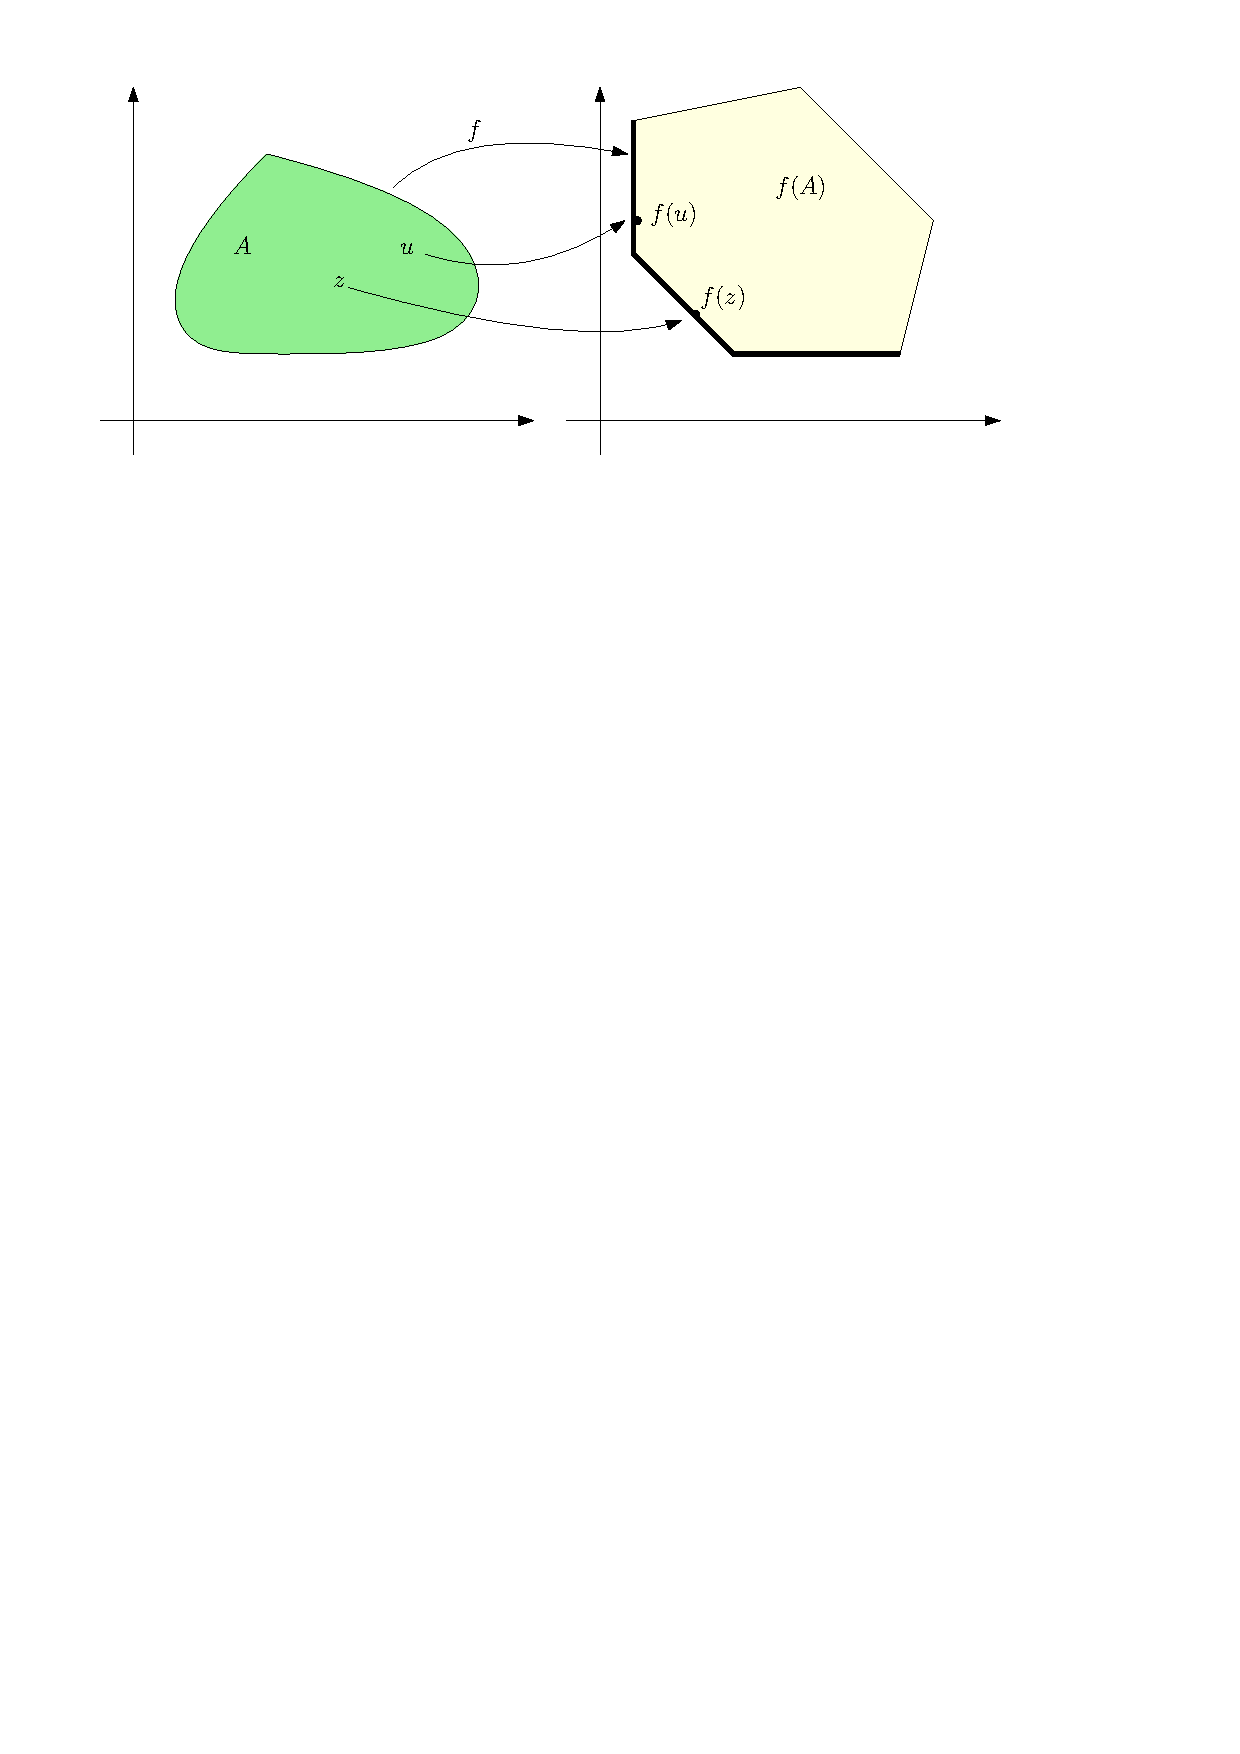
\includegraphics[width=0.9\linewidth]{nghiemtoiuu}
\caption{Nghiệm Pareto và Pareto yếu}
\end{center}
\end{figure}




\chapter*{Kết luận}                         % Chương 3
\addcontentsline{toc}{chapter}{{\bf  Kết luận}\rm}
\indent
\thispagestyle{fancy}

Luận văn này đạt được các vấn đề sau đây:

\begin{itemize}
	\item Tìm hiểu cách vô hướng hóa bài toán tối ưu theo các phương pháp khác nhau. Từ đó việc tìm nghiệm của bài toán tối ưu đa mục tiêu có thể được tìm kiếm thông qua bài toán tối ưu dạng vô hướng.
	\item Với mỗi phương pháp được khảo cứu, luận văn tìm hiểu được các mối quan hệ nghiệm giữa bài toán đa mục tiêu và bài toán vô hướng hóa.
	\item Ngoại trừ Ví dụ 2.1, các ví dụ trong luận văn do chúng tôi đề nghị để minh họa mối quan hệ nghiệm giữa bài toán đa mục tiêu và bài toán vô hướng hóa.
	
\end{itemize}



\begin{thebibliography}{99}
	\addcontentsline{toc}{chapter}{{\bf  Tài liệu tham khảo}} 
	\thispagestyle{fancy}
%	\item[\textbf{\large 1.}] \textbf{\large Tài liệu tham khảo chính thức}
	
	%\item[\textbf{\large 1.}] \textbf{\large Tài liệu tham khảo chính thức}
	
	
	%Các tài liệu chính được tôi chọn lựa để tham khảo khi thực hiện luận văn là  tài liệu số \cite{Mat}, \cite{Gab1} và \cite{Gian}. 	Các vấn đề liên quan được chúng tôi khảo cứu trong các tài liệu còn lại.
	
	\bibitem{Mat} M. Ehrgott, {\it Multicriteria Optimization}, Springer, 2005.
	
	\bibitem{Gab1} G. Eichfelder, {\it Adaptive Scalarization Method in Multiobjective Optimization}, Springer, 2008.
	
	\bibitem{Sonkim} T.Q. Son and D.S. Kim, {\it  $\epsilon$-Mixed type duality for nonconvex multiobjective programs with an infinite number of constraints}, Journal of Global Optimization 57,  447-465, 2013.
	
	
\end{thebibliography}

\end{document}







